%this is the DQC1 presentation

\documentclass{article}
\usepackage{etex}
\usepackage{amsmath}
\usepackage{amsthm}
\usepackage{braket}
\usepackage{tikz}
\usepackage{braids}

\begin{document}
\title{Explicit calculation of all the terms from the DQC1 paper, considering the Hopf link} 
\author{Ohad Barta}
\date{\today} 

\titlepage
\tableofcontents









\section{introduction}
In this document, we will see all the relevant calculations (knots, braids, Templey-Lieb algebra's, Markov Trace, Fibonacci representation), for the hopf link knot, which is shown in Figure 1.

\begin{figure}
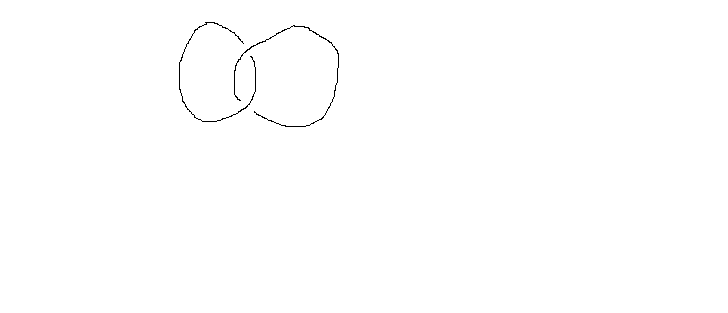
\includegraphics[scale=1]{raw_hopf_link} 
\caption{our knot of interest - the hopf link}
\end{figure}

\section{The hopf link Jones polynomial}

\subsection {The Hopf link kaufmann polynomial}
Recall the following definition of Kaufmann polynomaial. This section is copied from our full-version paper, including some simple examples of Kaufmann polynomials for simpler knots.

The last example in this section as you may see, is calculation of the Kaufmann polynomial for our hopf link.

\subsection{The Kaufmann polynomial definition}
Consider a knot K. for each crossing in K, from the form 
\begin{center}
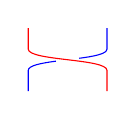
\begin{tikzpicture}
\braid[rotate=0, height=.3cm, style strands={1}{ red } ,style
strands={2}{ blue } ] s_1;
\end{tikzpicture}
\end{center} 

We decide at random to replace it with one of two options:
\begin{itemize}
\item One of the strands goes to the right, the other one remains on the left (considered choice 1 in the case that the upper-left strand was originaly "above" the other one, like in the picture above. considered choice "2" in case that the "upper-right" strand was originally above the other strand (i.e. if the blue strand was above the red one)
\item One of the strands remains on the top, the other strand remains at the bottom (considered choice 2 in the case that the left strand was originaly "above" the right one,  like in the picture above considered choice "1" in case that the "right" strand was originally above the left strand(i.e. if the blue strand was above the red one))
\end{itemize}
Each decision like this for all the crossings is a state \(\sigma\)

\begin{figure}
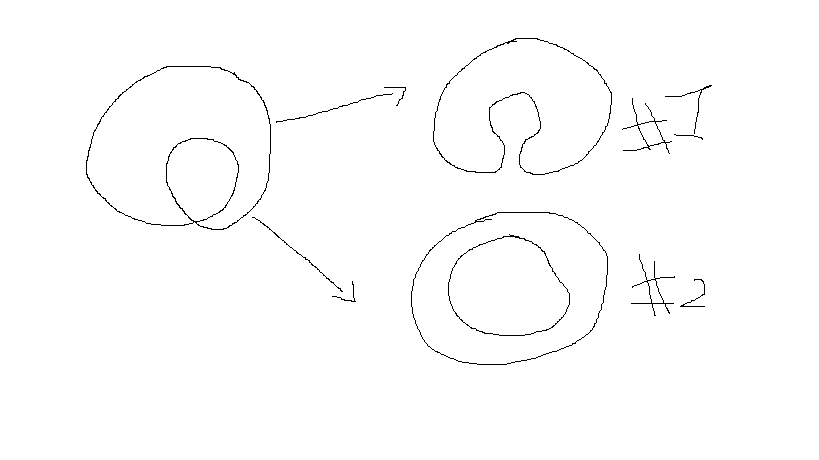
\includegraphics[scale=0.2]{kauffman_calc} 
\caption{kaufmann bracket example}
\end{figure}

We denote by \(\sigma_{+}\) the number of replaces we made choice 2, and by 
\(\sigma_{-}\) the number of replaces we made choice 1.
We denote by\(N_{\sigma}\) the number of loops created when all the changes of \(\sigma\) are applied.
The Kaufmann Bracket Polynomial is defined as:
\( L(A) = \sum\limits_{all_states_\sigma}{A^{\sigma_{+} -\sigma_{-}}d^{N_{\sigma} - 1}}\)

when:
\begin{itemize}
\item L stands for the Kaufmann polynomial.
\item A is a point that we want to evluate this polynomial at.
\item d is defined as \(d = -A^{-2} -A^2\) 
\end{itemize}

\subsection{Kaufmann polynomail simple examples}
\begin{itemize}
\item \(\forall A\), L(A)=1 in the unknot:
    \begin{itemize}
    \item we have only one state $\sigma$, with \(\sigma_{+}=0,\sigma_{-}=0\)
    \item this state have one loop, so \(N_{\sigma} = 1\)
    \item Therefore, $L(A) = A^{0}d^{0}=1$
    \end{itemize}
\item For two unknots:
    \begin{itemize}
    \item we have only one state $\sigma$, with \(\sigma_{+}=0,\sigma_{-}=0\)
    \item this state have two loops, so \(N_{\sigma} = 2\)
    \item Therefore, $L(A) = A^{0}d^{1}=d=-A^{-2}-A^{2}$
    \end{itemize}
\end{itemize}

\begin{figure}
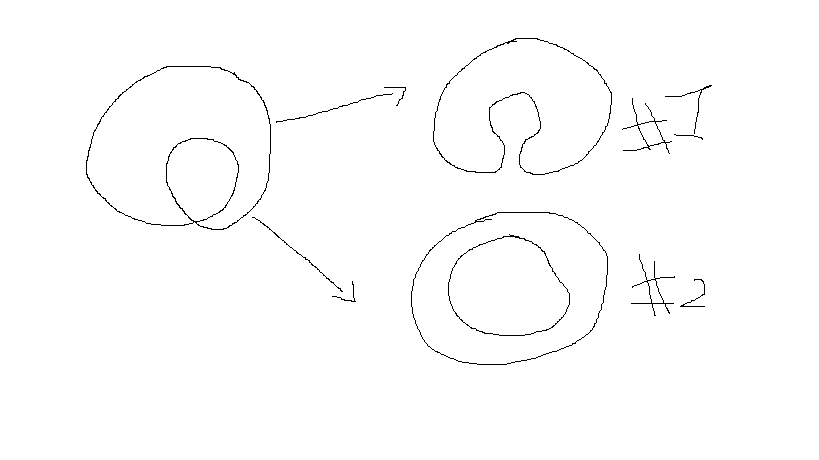
\includegraphics[scale=0.17]{kauffman_calc}
\caption{kaufmann polynomial, third example}
\end{figure}

Lets now exmine a bit more complicated case, as shown in Figure 2. Notice that at the intersection, the upper-left strand is above, and that this fact does matter.
\begin{itemize}
    \item we have two states. In choice 1, $\sigma_{-}=1$, In choice 2,$\sigma_{+}=1$
    \item If we chooce choice 1 we have \(N_{\sigma} = 1\), if we choose choice 2 we have \(N_{\sigma} = 2\)
    \item Therefore, $L(A) = A^{-1}d^{0} + A^{1}d^{1} = A^{-1} +A^{1}(-A^{-2}-A^{2}) = -A^{3}$
\end{itemize}

\begin{figure}
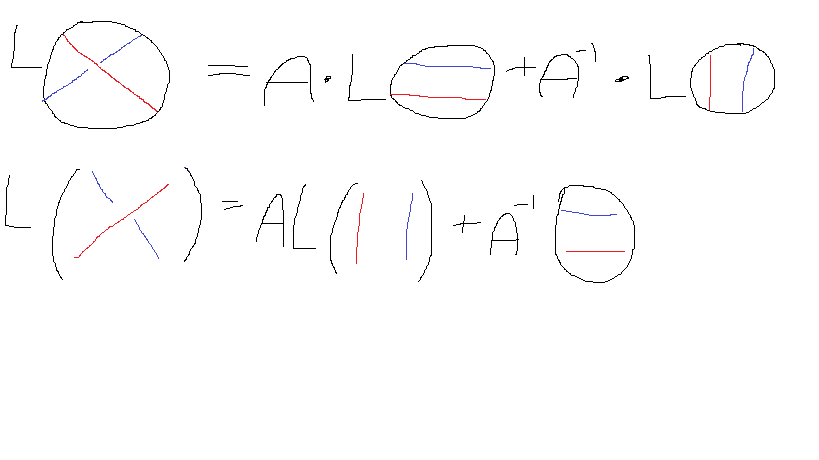
\includegraphics[scale=0.2]{kauffman_bracket_identity} 
\caption{kaufmann polynomial, recursive formula}
\end{figure}

\subsubsection{The Kaufman polynomial recursive formula}

The recursive formula for calculating the Kaufman polynomial is described at Figure 4. (Red strand above blue)
The formula comes directly from the definition, if we consider only one cross. We can use it to simplify the calculation of some more complicated knots (no need to track explicitly  $\sigma_{-}, \sigma_{+}, N_{\sigma}$).

Note, However, that this formula means that the number of elements in the polynom is exponential in the number of crosses.

Finally, the Kaufmann polynom calculation for out hopf link is described at figure 5.
\begin{figure}
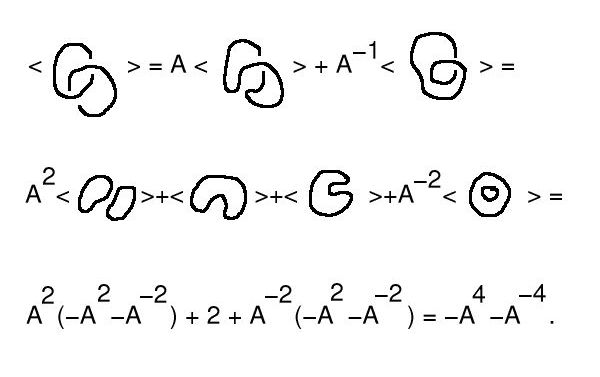
\includegraphics[scale=0.2]{hopf_link} 
\caption{the kaufmann polynomial of the Hopf link}
\end{figure}


\subsection{The Jones polynomial of the Hopf link}
Recall the following definition of Jones polynomial of a knot : 

We define by the w(k) for a knot k to be: \(w(k) = \sum\limits_{all crossings}{(-1)^{is the left arrow above the right one}}\)
and Jones polynomial is defines as: \(V_{k}(t)=V_{k}(A^{-4})=(-A)^{3w(k)}L_{k}(A)\).

Notice that w(k) for the unknot is 0, so the Jones polynomial of the unknot is still equals to 1 at any point.

Consider the Hopf link.

Moving to Jones Polynomial, we can see that w(HopfLink)=-2 (two cross with the same oreintation), so:
\(V_{hopfLink}=(-A)^{-6}(-A^{-4}-A^{4}) = -A^{-2} - A^{-10}\).
Remember that \(t = A^{-4}\) and we get \(V_{hopfLink}(t)=-\sqrt{t}(1+t^{2})\)  


Notice that the difference between the Jones and Kaufmann polynomial is only an easy-to-compute normalization factor. Therefore, we might show that some values (Markov trace, Fibonacci representation) are related to the kaufmann polynomial, they must also relate to the Jones polynomial, up to that factor.

\section{"The Markov trace of the Hopf link"}
First, why use quotes? Because recall that markov trace is defined over Templey-Lieb algebra objects, so first, we will have to figure out what the corresponding templey-lieb object is.

\subsection{The corresponding braid}

As the first step, we will have to find the braid b such that $b^{tr}$ equals to the hopf link. After a carefull visual observation we find out that the braid is 
\begin{center}
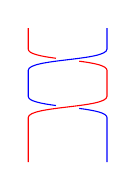
\begin{tikzpicture}
\braid[rotate=0, height=.3cm, style strands={1}{ red } ,style
strands={2}{ blue } ] s_1^-1 s_1^-1;
\end{tikzpicture}
\end{center} 

If we will "complete" this braid to its trace closure, we will the knot shown in Figure 6.
\begin{figure}
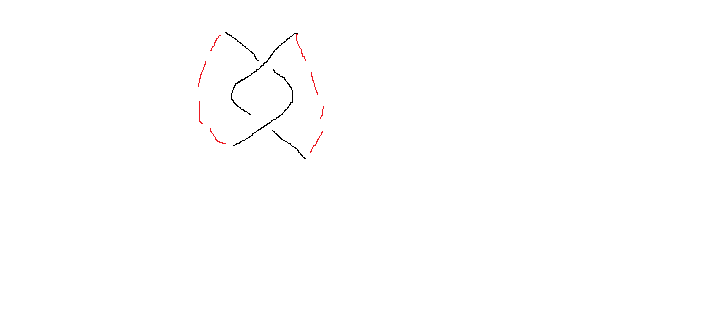
\includegraphics[scale=0.7]{braid_of_hopf_link} 
\caption{the kaufmann polynomial of the Hopf link}
\end{figure}

Recall that this is indeed the hopf link knot.

So, we know how the braid looks like, but what is this braid mathematically? Recall the braid generators definition (imported from the full version papaer) : 

$\forall 1\leq i \leq n$, we denote by $\sigma_{i}$, the braid which takes the i-th strand
to the (i+1) place, the (i+1)-strand to the i-th place, and leaves all the other strands in place.(the (i)th strand will be above in the collision area) 
For example, this is $\sigma_{2}$ with 3-strands:
\begin{center}
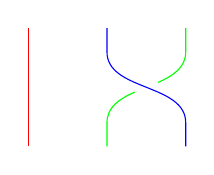
\begin{tikzpicture}
\braid[rotate=0, style strands={1}{ red } ,style
strands={2}{ blue } ,style strands={3}{ green } ]s_2;
\end{tikzpicture}
\end{center}

For each braid group generator, we define its inverse element to be the element which takes the i-th strand
to the (i+1) place, the (i+1)-strand to the i-th place, and leaves all the other strands in place. (the (i+1)th strand will be above in the collision area).

Following this definition, its easy to see that the braid we got (i.e. : \begin{center}
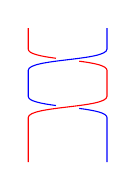
\begin{tikzpicture}
\braid[rotate=0, height=.3cm, style strands={1}{ red } ,style
strands={2}{ blue } ] s_1^-1 s_1^-1;
\end{tikzpicture}
\end{center} )
is $\sigma_{1}^{-1}\sigma_{1}^{-1}$ = $\sigma_{1}^{-2}$

\subsection{Templey-Lieb algebra reminder}
Recall the definition of the Templey - lieb algebra 
Temperley Lieb[n,d] algebra is ab algebra over the field of polynomials with coeffients in Z, such that:

There exists generators $E_{1}....E_{n-1}$, that obeys the following rules:
\begin{itemize}
\item \(E_{i}E_{j} = E_{j}E_{i}\), when \(2 \leq |i-j|\)
\item \(E_{i}E_{i+1}E_{i} = E_{i}\), \(E_{i}E_{i-1}E_{i} = E_{i}\)
\item \({E_{i}}^2 = dE_{i}\)
\end{itemize}

Each Temperley-Lieb element can be obtained as multiplication of these generators.

We won't treat these generators as polynoms. Rather, we will work with "graphic visualization" of that algebra. Graphically, the temperely-Lieb algebra defined as follows:
Tempely Lieb {n,d} algebra group consists of two rows of pegs (button and top), and n-strands, such that:
\begin{itemize}
\item each strand connects to exactly two pegs (but they can be from the same side!)
\item the strands cannot intersect between them.
\end{itemize}

In Figure 7 you can see an example to some Temerley-Lieb algebra objects
\begin{figure}
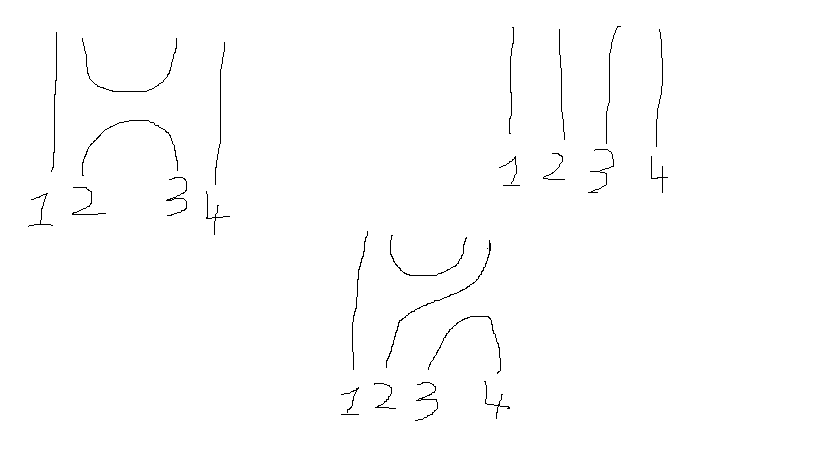
\includegraphics[scale=0.25]{tempely_lieb_generators} 
\caption{tempely lieb objects example}\
\end{figure}

Under this definition, the i-th Temperley-Lieb algebra generator will be the object which sends each bottom/top peg to is equivalent in the other row, except the i-th and the (i+1)th pegs : the top ith peg will go to the (i+1)th-top peg, and the ith bottom peg will go to the (i+1)th bottom peg. Notice that an example to generators can also be seen in Figure 7: the first picture there is of $E_{2}$ - the second generator.

The operation on 2 Templey-Lieb object is a simple contanenation. in case that a circle is created, it is removed, and we multiply the object by d (Recall that all the objects are actually polinomials, and this is only graphic view of them, so multiply by d is a well-defined action).

Figures 8-10 show examples to the action between templerley-Lieb objects, and also proves that this graphic representation obeys the 3 rules about the Temperley-Lieb generators.
\begin{figure}
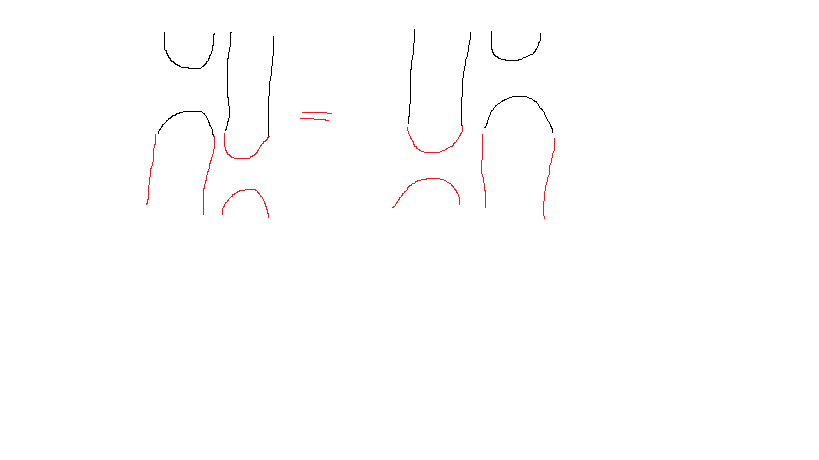
\includegraphics[scale=0.5]{tempely_lieb_first_rule} 
\caption{$E_{1}E_{3}=E_{3}E_{1}$}\
\end{figure}

\begin{figure}
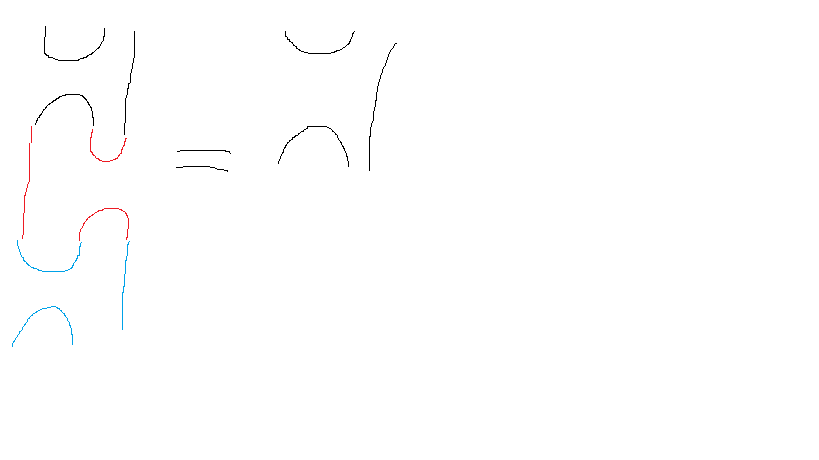
\includegraphics[scale=0.5]{tempely_lieb_second_rule} 
\caption{$E_{1}E_{2}E_{1}=E_{1}$}\
\end{figure}

\begin{figure}
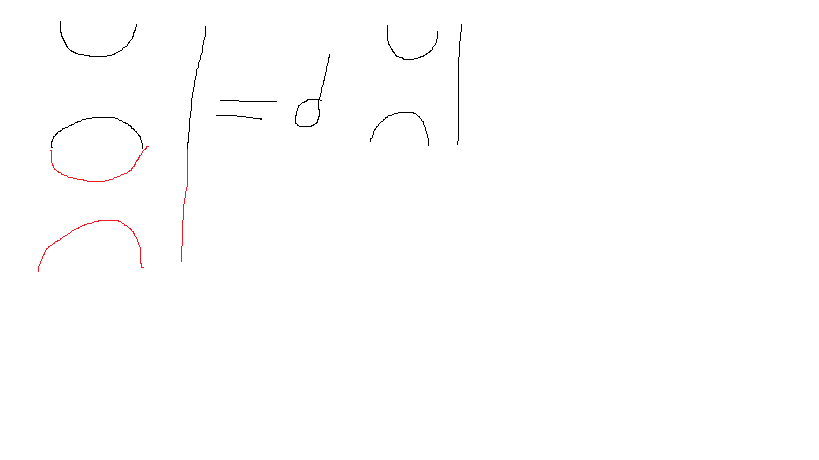
\includegraphics[scale=0.5]{tempely_lieb_third_rule} 
\caption{$E_{1}E_{1}=dE_{1}$}\
\end{figure}



\subsection{Our templey-Lieb object}
Now, lets see what is the Templey-Lieb algebra object which corresponds to the hopf link.
Moving to the Templey lieb object, recall the homomorphism we defined from braid groups to the Templey Lieb elements:
$\rho_{A}(\sigma_{i}) = AE_{i} +A^{-1}I$
(proof that this is indeed an homomorphism appears in the full version).

Recall that our braid group element was  $\sigma_{1}^{-2}$, so we have to calculate $\rho_{A}(\sigma_{1}^{-2})$.

First, lets try to figure out how $\rho_{A}(\sigma_{1}^{-1})$ will look like.


We know that $\rho_{A}(\sigma_{1}) = AE_{1} +A^{-1}I$. We also know that this is homomorphism, so  $\rho_{A}(\sigma_{1})\rho_{A}(\sigma_{1}^{-1}) = I$.

There are only 2 elements in Templey-Lieb(2,d) algebra : $E_{1}$ and I. Therefore, the most general form $\rho_{A}(\sigma_{1}^{-1})$ will get is :
$xE_{1} + yI$.

It should hold that $( AE_{1} +A^{-1}I)(xE_{1} + yI)$ = I.
From here we get two equations in x,y:
$ A^{-1}yI = I$, therefore $y=A$
$AxE_{1}^{2}+AyE_{1} + A^{-1}xE_{1} = 0$. After instantiating y, and recalling that $E_1^{2} = dE_{1}$, we get :  
$AdxE_{1}+A^{2}E_{1} + A^{-1}xE_{1} = 0$, after instantiating $d=-A^{-2} -A^{2}$ we get 
$-A^{-1}xE_{1} - A{3}xE_{1} +A^{2}E_{1} + A^{-1}xE_{1} = 0$, or $x=A^{-1}$.

Therefore,  $\rho_{A}(\sigma_{1}^{-1}) = A^{-1}E_{1} + AI$

Finally, we get that our Templey-Lieb object will be:
$\rho_{A}(\sigma_{1}^{-2}) $ = $(\rho_{A}(\sigma_{1}^{-1}))^{2}$ = $(A^{-1}E_{1} + AI)^{2}

\subsection{The Markov trace function of our Templey-Lieb object}

First, recall the definition of the Markov trace:
The Markov Trace is a function on a Temperley-Lieb algebra, which defined as follows:
\begin{itemize}
\item given a Temperley-Lieb algebra object, we connect its bottom and top bars, in a similar way to
a trace closure.
\item when denote the number of loops created like this with a, the trace closure is $d^{a-n}$
\end{itemize}.

example to the computation of the Markov trace with $E_{1}$ with 3 strands, can be found in Fig. 11.
\begin{figure}
\centering
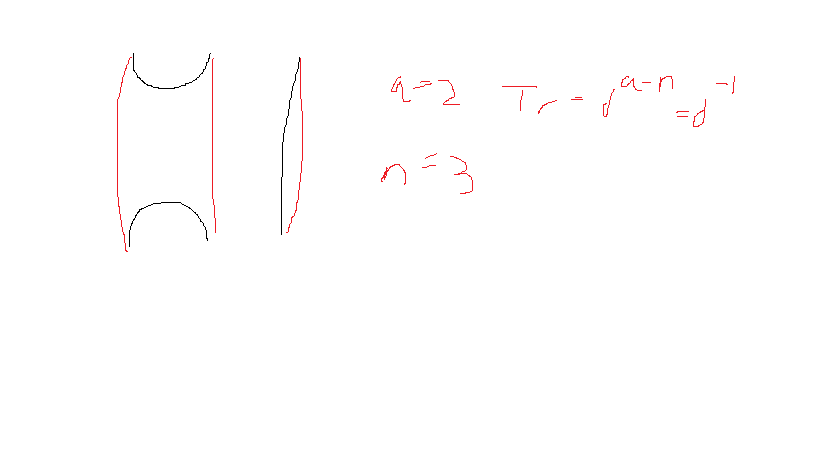
\includegraphics[scale=0.25]{MarkovTraceExample}
\caption{example of calculation of the markov trace function}
\label{fig:my_label}
\end{figure}


From the definition, we can easily conclude that in our Templey-Lieb[2,d] algebra, it holds that $Tr[E_{1}] = d^{-1}$, $Tr[I] = 1$.


Moving to the calculation of the Markov trace of Hopf-link "Templey-Lieb object" we get: 
$Tr[ (A^{-1}E_{1} + AI)^{2}] = Tr[ (A^{-2}E_{1}^{2} + 2E_{1} + A^{2}I)] =  Tr[ (A^{-2}dE_{1} + 2E_{1} + A^{2}I)] =  Tr[ (-A^{-4}E_{1} + E_{1} + A^{2}I)]$ , which in turn equals to: 
$Tr[ (-A^{-4}E_{1} + E_{1} + A^{2}I)] = \frac{1 - A^{-4}}{d} + A^{2}$

\subsection{Show the relation between the Markov Trace and the Kaufmann polynomial}

In the lecture, we claimed that:
\begin{theorem}
Let B be some braid group element. Let $B^{tr}$ denote the knot we get from B by the trace closure method. Recall the additional, already defined, notations:
\begin{itemize}
\item V - The Jones polynomial.
\item $\rho_{A}(B)$ = the Templey-Lieb algebra we get by apply the homomorphism $\rho_{A}$ on the braid B.
\item w - the Jones polynomial normaization factor
\item $d = -A^{2}-A^{-2}$
\item Tr- The Markov Trace function
\end{itemize}

Then it holds that
$V_{B^{tr}}(A) = (-A)^{3w(B^{tr})}d^{n-1}Tr[\rho_{A}(B)]$

Lets show that this theorem holds in this case.

What we actually need to show is that $L_{B^{tr}}(A) = d^{n-1}Tr[\rho_{A}(B)]$, when L is the kaufmann polynomial.

We saw that L(HopfLink) = $-A^{-4}-A^{4}$.
On the other hand, it holds that $d^{2 - 1}Tr[\rho_{A}(B)]$ = $d( \frac{1 - A^{-4}}{d} + A^{2})$ = $1 - A^{-4} -1 -A^{4} = -A^{-4}-A^{4}$

And we got equal expressions, as required.

\section{The Fibonacci representation, and the correlation to Jones Polynomial} 

\subsection{The Fibonacci representation - reminder}
Here, in addition to the definition of the Fibonacci represetation, I included some intuition regarding to what its idea is. 
We already know that braids are an easy way to represent a knot. But eventually we will have to come up with a quantom algorithm that works on matrices.

Such matrix representation must have some properties that will make it useful to us:
\begin{itemize}
\item for every braid, its matrix must be unitary, so we can link it to some quantom circuit.
\item for every braid, there has to be some connection between the Jones Polynomial of the braid, and the relevant matrix.
\end{itemize}

 So, how we represent a braid as a matrix?
 
As a first intuition, we would expect that the representation of the identity braid will be the identity matrix. This intuition, although seems simple and clear, gives us a clue about our representation method: We will match each crossing in the braid some "little matrix", and the general representation will be the multiplication of all these matrices.

Next, lets attend to a question with less intuitive answer: what is the dimension of this matrix should be? clearly, the dimension should grow with the braid size, however the naive approach of multiply the matrix dimension for each new braid, sounds like a waste.

 Given an n-strand braid, we can write a string of n+1 elements on the bottom of the braid between every two strands, where each element is either * or p. The only restriction is that there will be no two adjacent * elements. The number of possibilities to do so is of course $f_{n+3}$, where $f_{n}$ denotes the $n$th Fibonacci number.

Next, for each crossing and labelling of it (the 3 elements from the right, left, and in the crossing) , we would like to give a linear function (i.e. - a row in the matrix) that will "represent" the crossing, and that may change the center label. (we wouldn't want to change the right or left label, in order to preserve the string of elements correctness under all the operations).

That is, in the most general form, a cross $\sigma_{i}$ with labeling of P*P, can move to 
a times the Identity with labelling P*P + b times the identity with labelling PPP.
we will denote it by $(p\hat{*}p)=a(p*p)+b(ppp)$

Lets take a look on the explicit, formal representation, and them see some examples:

$(*\hat{p}p)=a(*pp)$

$(*\hat{p}*)=b(*p*)$

$(p\hat{*}p)=c(p*p)+d(ppp)$

$(p\hat{p}*)=a(pp*)$

$(p\hat{p}p)=d(p*p)+e(ppp)$

, with:
$ a = -A^{4} $


 $  b = A^{8}  $
 
 $  c = A^{8}\tau^{2} - A^{4}\tau $
  
 $  d = A^{8}\tau^{\frac{3}{2}} + A^{4}\tau^{\frac{3}{2}} $ 
 
 $  e = A^{8}\tau - A^{4}\tau^{2} $ 
 
 $  A = e^{\frac{-3{\pi}i}{5}} $ 
 
 $  \tau = \frac{2}{1 + \sqrt{5}} $


 
\subsection{The Fibonacci representation - examples}
First, notice that indeed, the representation of the identity braid, is the identity matrix. Next, lets show the representation of $\sigma_{1}$, with 2 strands. The dimension of the matrix should be $f_{2+3}=f_{5}=5$. The matix itself will be:

\begin{pmatrix}
b & 0 & 0 & 0 & 0 \\ 0 & a & 0 & 0 & 0 \\ 0 & 0 & a & 0 & 0 \\ 0 & 0 & 0 & c & d \\ 0 & 0 & 0 & d & e 
\end{pmatrix}
\begin{pmatrix} *p* \\ *pp \\ pp*\\ p*p \\ ppp
\end{pmatrix}

Next, We will show the Fibonacci representation of $\sigma_{1}$ with 3 strands:
\[
\begin{pmatrix} b & 0 & 0 & 0 & 0 & 0 & 0 & 0 \\ 0 & a & 0 & 0 & 0 & 0 & 0 & 0 \\ 0 & 0 & a & 0 & 0 & 0 & 0 & 0 \\ 0 & 0 & 0 & e & 0 & 0 & 0 & d \\ 0 & 0 & 0 & 0 & a & 0 & 0 & 0 \\ 0 & 0 & 0 & 0 & 0 & e & d & 0 \\0 & 0 & 0 & 0 & 0 & d & c & 0 \\0 & 0 & 0 & d & 0 & 0 & 0 & c \end{pmatrix} 
  \begin{pmatrix} *p*p \\ *ppp \\ *pp* \\ pppp \\ pp*p \\ ppp* \\ p*p* \\ p*pp \end{pmatrix}
\]


Now, We will show the Fibonacci reoresentation of $\sigma_{2}$ with 3 strands:
\[
\begin{pmatrix} c & d & 0 & 0 & 0 & 0 & 0 & 0 \\ d & e & 0 & 0 & 0 & 0 & 0 & 0 \\ 0 & 0 & a & 0 & 0 & 0 & 0 & 0 \\ 0 & 0 & 0 & e & d & 0 & 0 & 0 \\ 0 & 0 & 0 & d & c & 0 & 0 & 0 \\ 0 & 0 & 0 & 0 & 0 & a & 0 & 0 \\0 & 0 & 0 & 0 & 0 & 0 & b & 0 \\0 & 0 & 0 & 0 & 0 & 0 & 0 & a \end{pmatrix} 
  \begin{pmatrix} *p*p \\ *ppp \\ *pp* \\ pppp \\ pp*p \\ ppp* \\ p*p* \\ p*pp \end{pmatrix}
\]

And what about the representation of $\sigma_{1}\sigma_{2}$ with 3 strands? In that case , we will just multiply the matrices from the both previous examples.

\subsection{The Fibonacci representation of our braid}

Recall that the braid corresponding to our hopf link was $\sigma_{1}^{-2}$. We already computed the fibonacci representation of $\sigma_{1}$ in the prev section. The Fibonacci representation of $\sigma_{1}^{-1}$ will be of course the inverse matrix. Since the Fibonacci representation matrices are unitary (proof full that - in the full paper!), the inverse matrix is simply $U^{\dagger}$, or: $\rho_{f}(\sigma_{1}^{-1}) = $
\begin{pmatrix}
$b^{\dagger}$ & 0 & 0 & 0 & 0 \\ 0 & $a^{\dagger}$ & 0 & 0 & 0 \\ 0 & 0 & $a^{\dagger}$ & 0 & 0 \\ 0 & 0 & 0 & $c^{\dagger}$ & $d^{\dagger}$ \\ 0 & 0 & 0 & $d^{\dagger}$ & $e^{\dagger}$
\end{pmatrix}
\begin{pmatrix} *p* \\ *pp \\ pp*\\ p*p \\ ppp
\end{pmatrix}

For getting the representation of our braid, we have: $\rho_{f}(\sigma_{1}^{-2}) = \rho_{f}(\sigma_{1}^{-1})\rho_{f}(\sigma_{1}^{-1})$ = 
\begin{pmatrix}
$b^{\dagger}$ & 0 & 0 & 0 & 0 \\ 0 & $a^{\dagger}$ & 0 & 0 & 0 \\ 0 & 0 & $a^{\dagger}$ & 0 & 0 \\ 0 & 0 & 0 & $c^{\dagger}$ & $d^{\dagger}$ \\ 0 & 0 & 0 & $d^{\dagger}$ & $e^{\dagger}$
\end{pmatrix}\begin{pmatrix}
$b^{\dagger}$ & 0 & 0 & 0 & 0 \\ 0 & $a^{\dagger}$ & 0 & 0 & 0 \\ 0 & 0 & $a^{\dagger}$ & 0 & 0 \\ 0 & 0 & 0 & $c^{\dagger}$ & $d^{\dagger}$ \\ 0 & 0 & 0 & $d^{\dagger}$ & $e^{\dagger}$
\end{pmatrix}

which equals to:
\end{pmatrix}\begin{pmatrix}
$(b^{\dagger})^{2}$ & 0 & 0 & 0 & 0 \\ 0 & $(a^{\dagger})^{2}$ & 0 & 0 & 0 \\ 0 & 0 & $(a^{\dagger})^{2}$ & 0 & 0 \\ 0 & 0 & 0 & $(c^{\dagger})^{2} + (d^{\dagger})^{2}$  & ($d^{\dagger}c^{\dagger} +d^{\dagger}e^{\dagger}) $ \\ 0 & 0 & 0 &($d^{\dagger}c^{\dagger} +d^{\dagger}e^{\dagger})$ & $(e^{\dagger})^{2} + (d^{\dagger})^{2}$
\end{pmatrix}
\begin{pmatrix} *p* \\ *pp \\ pp*\\ p*p \\ ppp
\end{pmatrix}

\subsection{The correlation between the Jones polynomial and the Fibonacci representation}

Recall that we saw that the Kaufmann polynomial is $L(hopfLink) = -A^{-4} - A^{4}$. Its time to instantiate our A. $A=e^{\frac{-3i\pi}{5}}$.

Therefore,  $L(hopfLink)(e^{\frac{-3i\pi}{5}) = -e^{\frac{12i\pi}{5}} - e^{\frac{-12i\pi}{5}}$ = $e^{\frac{2i\pi}{5}} - e^{\frac{-2i\pi}{5}} = -0.618$

Now, recall the Trace function we defined over the Fibonacci representation : 

$\tilde{Tr} = \frac{1}{{\phi}f_{n}+f_{n-1}}\sum\limits_{s \in Q_{n+1}}{W_{s}}\rho_{f}(b)_{s,s}$.

when $\phi$ is the constant $\frac{1 + \sqrt{5}}{2} $, $\rho_{f}(b)_{s,s}$ denote the s-th diagonal entry in the Fibonacci representation of a braid b,
and $W_{s}$ is $\phi$ if s ends with p, and 1 if s ends with *. $Q_{n+1}$ is the set of all strings with length n+1 that obeys the "no two adjective *" rule, and in addition - starts with "*"!

In the lecture, we showed that this function behaves like the Markov trace, at the point A. Therefore, it should hold that $\tilde{Tr}(HopfLink)d = L(hopfLink)$ (We get here the d factor because the Markov trace has, see previous sections).



Time to instantiate.

Here, n=2, so $f_{n} = f_{n-1} = 1$. After combining this with the result of the Fibnocci representation from the previous section, we get:
$\tilde{Tr} =  \frac{1}{{\phi}+1}(Fib((\sigma_{1})^{-2})[*p*,*p*]+ {\phi}Fib((\sigma_{1})^{-2})[*pp,*pp]) = \frac{1}{{\phi}+1}((b^{\dagger})^{2} + \phi(a^{\dagger})^{2})$

(Notice that we have only 2 terms in the sum, for the two elements which start with "*").

After instantiation of a,b we get:
(remeber that A here is just another name for $e^{\frac{-3i\pi}{5}}$)
$\tilde{Tr} = \frac{1}{{\phi}+1}(A^{-16} + \phi A^{-8}}) = \frac{1}{{\phi}+1}(e^{\frac{-2{\pi}i}{5}} + \phi e^{\frac{4{\pi}i}{5}})$

when we remember to multiply this expression by $d = -A^{-2} - A^{2} = -e^{\frac{-6{\pi}i}{5}} -  e^{\frac{6{\pi}i}{5}}$ , we get -0.618 as our final result, which is equal to the kaufmann polynomial value, as required.


\end{document}